\section{System Architecture}
The system we have designed consists of two parts,
one being a input device
and the other being an application able to recognize the patterns from the device and forward predefined commands.

\subsection{The Input Device}
Our motion tracking device has been built in such a fashion that it resembles a wrist watch.
This form factor makes it rather compact.
Additionally a lot of people wear watches on a daily basis which makes it recognizable and barely noticeable for people.

The specific device contains a list of components, the most important are 6DoF Sensor, Bluetooth and Arduino microcontroller.

\textbf{6DoF Sensor:}\\
This is the heart of the device. It contains an accelerometer and a gyroscope. This means we can measure movement and rotation of the wrist of anyone wearing the device.

\textbf{Arduino Pro Mini:}\\
This is the brain of the device, it handles all communication between the 6DoF chip and forwards the data over bluetooth to any consumers of the data.

The others are not that important to spend a lot of time on, they provide means of communicating, charging and toggling the device on and off.

\begin{figure}[!h]
\centering
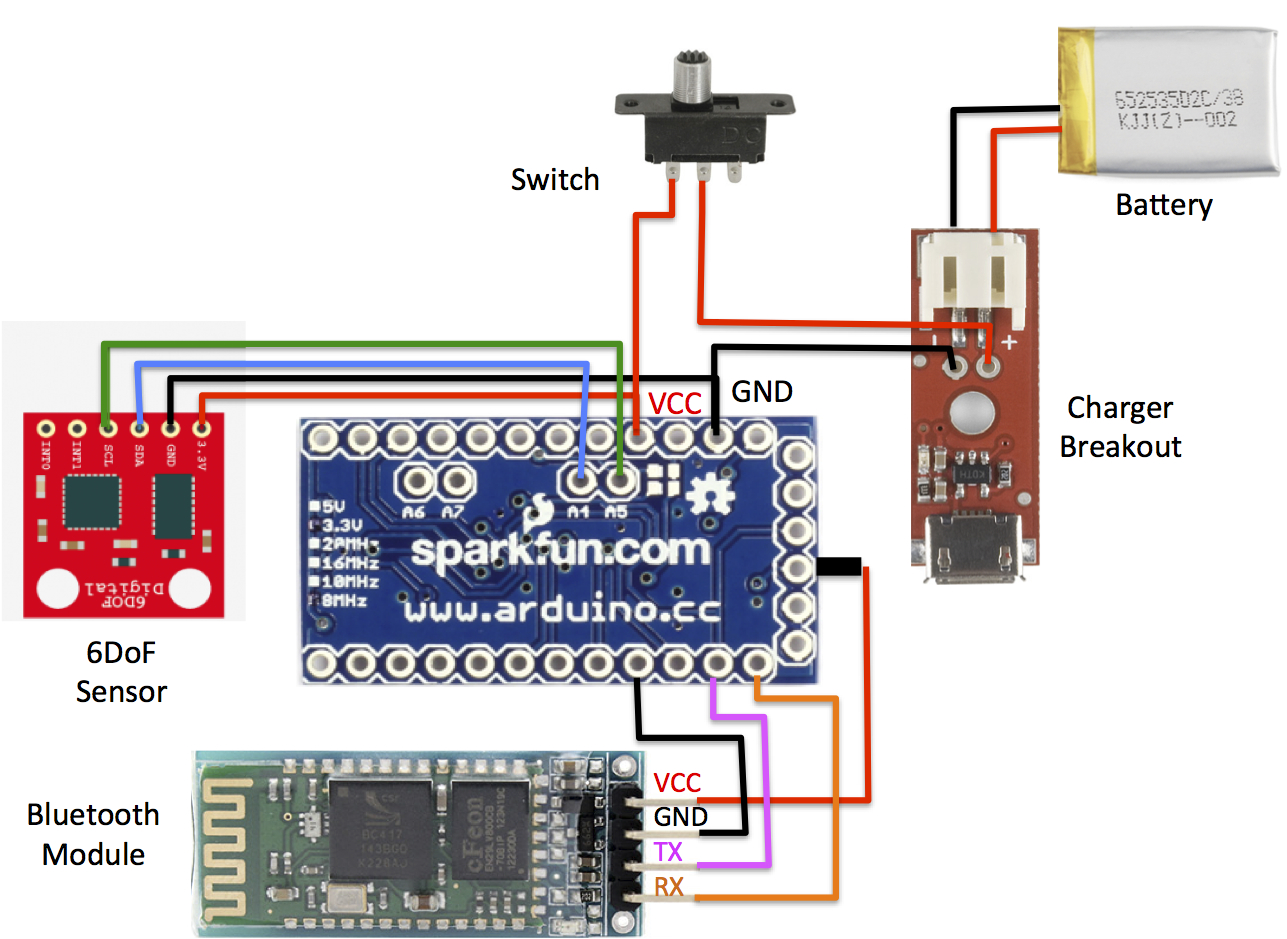
\includegraphics[width=0.9\columnwidth]{img/device_schematic}
\caption{This schematic shows the circuitry on the device.}
\label{fig:figure1}
\end{figure}

\subsection{Weka Gesture Recognition System}
Since the input device we have built is quite lightweight, data processing needs to be done elsewhere.
This provided us with the challenge of transferring data from one bluetooth capable device to another.
All the processing and preprocessing of the device's data is performed on a desktop application on a 
computer connected to the device.
Especially challenging was to find and use Java libraries that would allow to establish a Bluetooth 
connection with the device and to exchange data with the desktop application that would process it. 
For further technical details about the challenges encountered please refer to the Discussion section. 
\todo{add technical details about the rxtx fucking everything up}
Once the acceleration and rotation data is sent from the device to the computer,
 the values are smoothed with an average of the 20 previous values in order to avoid and reduce the effect of noise on the sensors.
 This phase is called preprocessing of the data. 
 This allowed us to have more precise information, and switch from this:

\begin{figure}[!h]
\centering
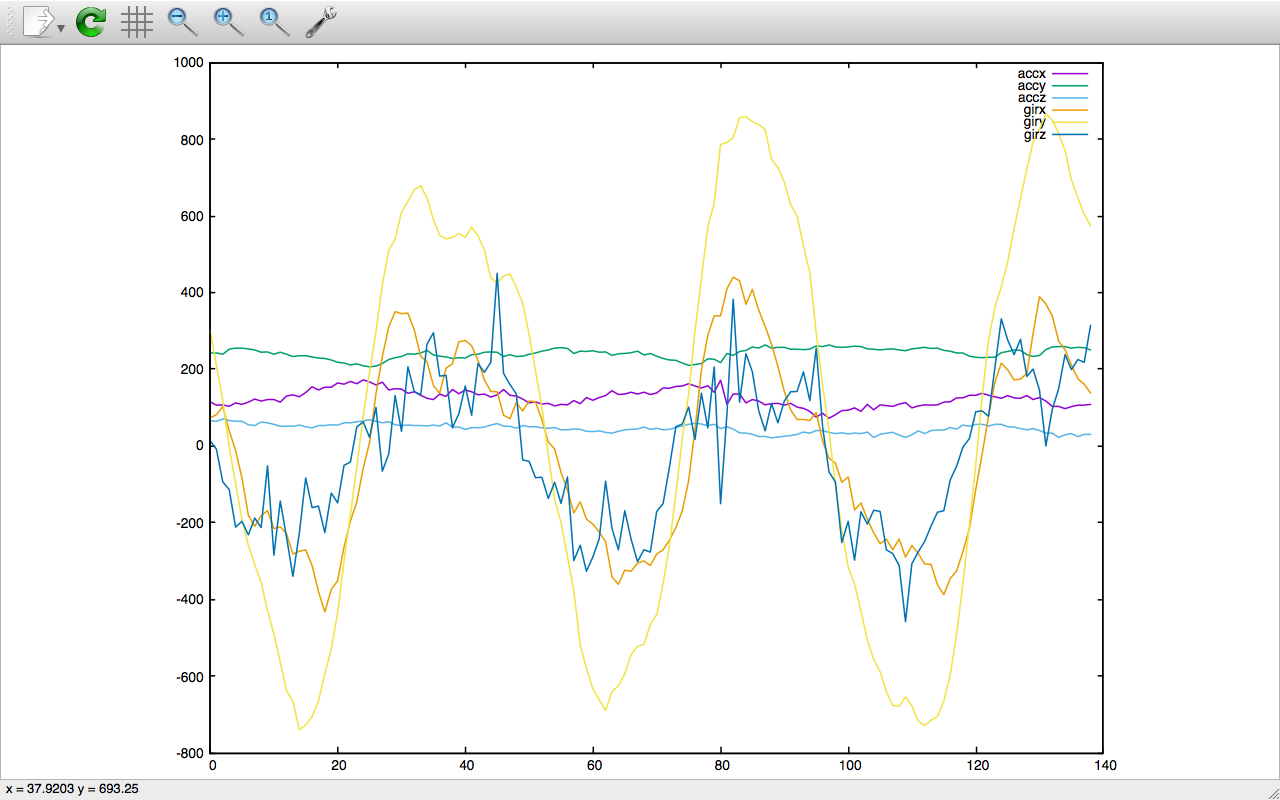
\includegraphics[width=0.9\columnwidth]{img/raw}
\caption{Data from the device before preprocessing.}
\label{fig:figure2}
\end{figure}

To this:

\begin{figure}[!h]
\centering
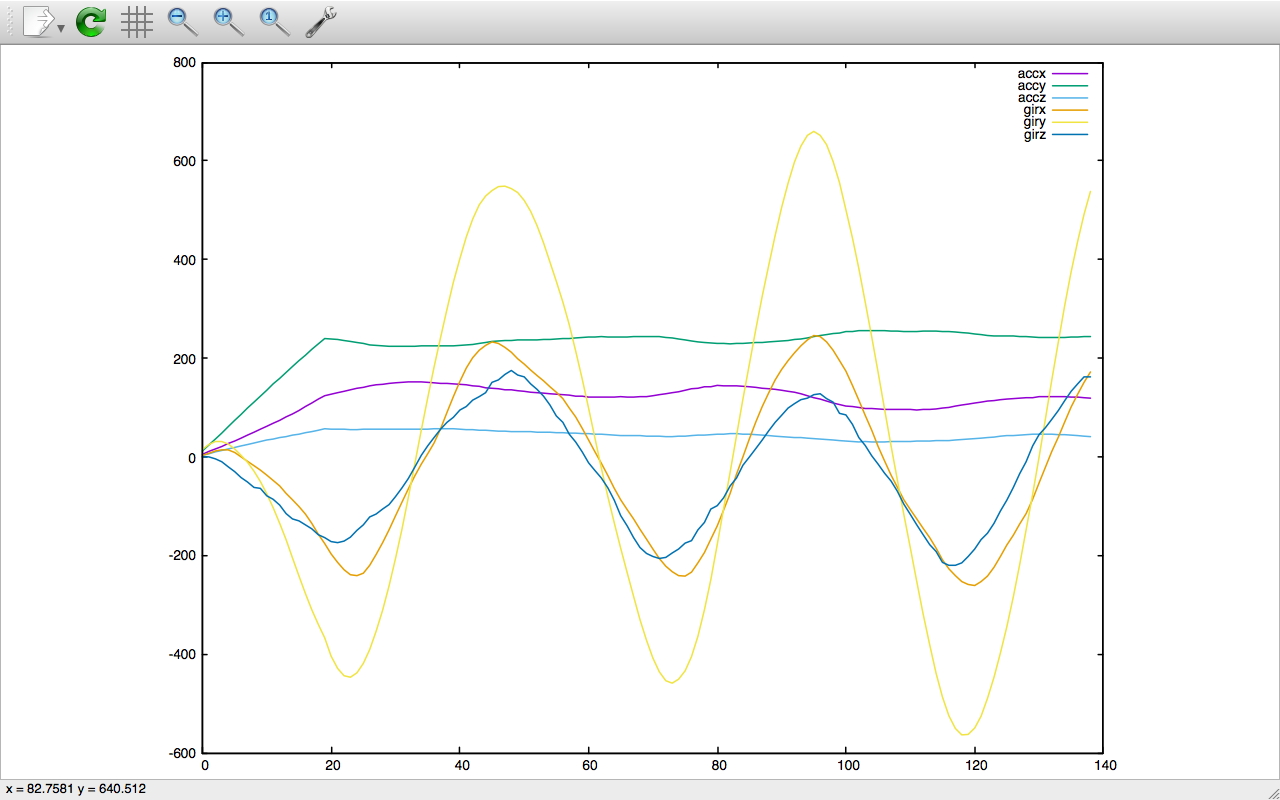
\includegraphics[width=0.9\columnwidth]{img/20}
\caption{Data from the device after preprocessing.}
\label{fig:figure3}
\end{figure}

For the actual processing and gesture recognition, we organized known gestures in a large training set, each individual gesture stored as a list of 50 * 6 values plus an identifier. 
We use Weka 3.6 to evaluate newly received data using a BayesNet classifier and comparing it to the training set.
The evaluation of the gesture is performed every 10 * 6 new values received.

\subsection{Android Application}

\subsection{Webservice}


\subsubsection{Pattern Recognition}